\documentclass[conference,10pt,times,letter]{IEEEtran}
\usepackage{blindtext, graphicx}
%\usepackage{timesnewroman}

% correct bad hyphenation here
\hyphenation{op-tical net-works semi-conduc-tor}

\newlength{\frameHeight}

\begin{document}
%
% paper title
% can use linebreaks \\ within to get better formatting as desired
\title{Biometric Patterns on Hooded Norway Rats}

% author names and affiliations
% use a multiple column layout for up to three different
% affiliations
\author{
\IEEEauthorblockN{Nils Napp, Yifang Liu \\ and Maira Saboia}
\IEEEauthorblockA{Department of  Computer Science and Engineering\\
University at Buffalo}
\and
\IEEEauthorblockN{Matthew J. Paul}
\IEEEauthorblockA{Department of Psychology\\ 
University at Buffalo}
}

% make the title area
\maketitle

\begin{abstract}
%\boldmath
%\blindtext[1]
bla bla bla
\end{abstract}
% IEEEtran.cls defaults to using nonbold math in the Abstract.
% This preserves the distinction between vectors and scalars. However,
% if the journal you are submitting to favors bold math in the abstract,
% then you can use LaTeX's standard command \boldmath at the very start
% of the abstract to achieve this. Many IEEE journals frown on math
% in the abstract anyway.

% Note that keywords are not normally used for peerreview papers.
\begin{IEEEkeywords}
Hooded Norway rats,  long-term tracking, rat dataset, behavior analysis.
\end{IEEEkeywords}

% For peer review papers, you can put extra information on the cover
% page as needed:
% \ifCLASSOPTIONpeerreview
% \begin{center} \bfseries EDICS Category: 3-BBND \end{center}
% \fi
%
% For peerreview papers, this IEEEtran command inserts a page break and
% creates the second title. It will be ignored for other modes.
\IEEEpeerreviewmaketitle

\section{Introduction}
%\blindtext


Long-term, minimally invasive, behavior analysis of animals has been a goal in the research community for some time. The reason is twofold; first, this type of automation allows for a more scalable, quicker and cost effective analysis of traditional video data. Second, it allows entirely novel types of analysis due to the novel scale duration and finer quantitative resolution of individual actions, for example high resolution pose estimates in addition to more easily distinguishable behaviors. For single animals and simple interactions excellent tools already exist, however social interactions between multiple individuals over longer periods of time still present significant challenges and is an active area or research~\cite{weissbrod2013automated}\cite{ohayon2013multiday}\cite{de2012computerized}.

Maintaining the identity of individual animals is one of the fundamental difficulties in this type analysis, since differences in behavioral state or tendencies toward certain actions are only useful if observations at one time can be reliably linked to a specific individual. In practice this problem is often posed as a tracking problem and solved via visual appearance or motion models to maintain identity between video frames and/or by adding identifying visual or radio frequency markers. In this paper we investigate the use of patterns in coloration of laboratory rats ({\it Rattus norvegicus}) of the Long-Evans strain as a biometric marker akin to fingerprints in humans. This strain has a distinctive "hood" pattern and is commonly used in behavioral cognitive studies, \cite{lambert2016natural,guarraci2016exposure,turner2014comprehensive}. In such studies consistent identity of multiple interacting individuals where interactions can lead to confusion are particularly interesting. 

The presented approach is related to the re-identification problem in visual tracking, but poses a slightly more general question about the identification quality of the marks themselves, i.e. if the coloration is a biometric marker~\cite{kuhl2013animal}. To be a good biometric marker, patters should be uniquely identifying between many individual rats taken in different times and conditions.
Good biometric markers would make any type of long term observation more reliable, as they could be used either directly for analyzing individual images, for re-identification during tracking, or could be used in parallel to tracking methods in order to check the long-term identity maintenance of visual tracking software. This complementary approach could be particularly useful in completely automated settings where independent identity measurements could be used for quality assurance.  
 
To answer the question of feasibility as a maker, we present a dataset of XX individual rats interacting in pairs, see Section~\ref{sec:dataset}, and give some initial results assessing the quality as a biometric marker, see Section~\ref{sec:results}. The concluding Section~\ref{sec:conclusion} discusses directions for future research. 

%Behaviour analisys is very important because of 
%\cite{weissbrod2013automated}.... 



%\cite{lambert2016natural,guarraci2016exposure,turner2014comprehensive}

%The Long-Evans rats (Hooded Norway rats) are commonly used in cognitive studies \cite{lambert2016natural,guarraci2016exposure,turner2014comprehensive}, frequently these experiments last several weeks or months, hence, especially when several individuals are placed in the same cage, keep tracking of each animal for a long period of time is a challenging task. In order to overcome this drawback usually, the animals are marked in the tail as in \cite{lambert2016natural}. However, the number of possible distinguishable markers is limited, therefore, with the increase in the number of individuals that share the same cage increases, this approach becomes impractical. 

%with a marker which sometimes need to be refreshed.

%\cite{noldus2001ethovision}

%Object identification. EthoVision distinguishes between two animals in the same arena on the basis of size. To distinguish two animals that are the same size, the user can partly color one animal to the same grayness as the background, thus reducing its apparent size (see Fig- ure 8). Color tracking can be used to distinguish more than two animals (up to 16 per arena). If the animals being tracked are the same color, markers can be used to paint blobs on the animals, which the system will be able to track. For more details on color tracking, see the “Object Detection” section above.

%Object detection. To ensure optimal object detection in any experimental setup, EthoVision offers three different object detection methods. Gray scaling is the fast- est. This method defines the animal as all connecting pixels that are both brighter than a low gray scale thresh- old and darker than a high threshold, and it defines the background as all other pixels. The thresholds can either be set manually by the user or be calculated automatically by the program. Gray scaling is a fast detection method (allowing the highest sample rate), but it cannot be used if the same gray scale values are present in both the ani- mal’s image and the background. The third detection method, color tracking, uses the color of the animal The second method, subtraction , first (before the start of the trial) makes a reference image, 

% cognitive experiments,

%In \cite{lambert2016natural} in order to keep tracking of the rats, each animal’s tail was marked with a nontoxic marker \cite{guarraci2016exposure}

%\cite{weissbrod2013automated} 

%To circumvent inherent human constraints, there is a critical need for machine-based tracking and behavioural phenotyping technologies that are applicable toward the analysis of socially interacting groups of animals. Several research teams have developed automated vision-based tracking tools that support behavioural phenotyping of a single individual in its home cage



%What is the problem?
%Why do we care about this problem?
%Is it possible to use the back patterns on hooded Norway rats as fingerprint ( to disguinsh them)?
%what should be a good approach?
%Is it useful for automatic behavior analysis?


\section{Related Work}


\subsection{Animal biometrics}
\label{sec:biometrics} 

\cite{kuhl2013animal} ...


\label{sec:related}

Given raw video data the task of automated behavior annotation has several technically challenging steps. First, the animals in the video data need to be located, and then potentially tracked and analyzed. These tracked data are the basis for quantitative behavior analysis. Depending on the animal species the video and behavior analysis have varying degrees of technical difficulty. Animals with uniform appearance, shape, and where to social interactions do not produce overlapping locations are much easier to track than highly deformable rodents. For example there has been considerable success in tracking and analyzing large volumes of fruit fly interactions

\subsection{Automated Behavior Analysis}
%Need to say that lont-term behaviorl obervation is still somehwat challaging 

%What are the challenges and how have others solved them?
Production grade open-source and commercial products exist for behavioral analysis in many different animal, e.g. CTrax~\cite{branson2009ctrax-fly} Noldus~\cite{noldus2001ethovision} \cite{de2012computerized}. These methods focus on ease of use and reliability. 

For Single animals in and simple social interactions they currently work well and enable high-throughput analysis even in highly deformable rodents~\cite{noldus2001ethovision}. Similarly many research groups that focus on machine learning and automating visual tasks have research developed (and published) code for specific applications and are studying how machine learning can be used to automate more behavioral scoring in which videos need to be segmented and scored e.g.~\cite{CRIM13}. 
% There are more papers by this group maybe pick one more.


\subsection{Object detection, Tracking, and Recognition}
Object detection, recognition, and tracking are closely related and a reliable automation tool will mix these conceptually distinct problems to achieve a reliable solution. The detection problem is to find instances in a video frame or image; the tracking problem is to associate detected instances in multiple video frames and to associate them; and the recognition problem is to identify individuals as being a specific entry from a previously known set. 
%(IS THIS TRUE?) 
Spatial relationships that arise from motion are one of the cues that are used to associate instances during tracking and in addition to resolve ambiguity most trackers also build some sort of appearance model of the tracked individuals in order to distinguish them in ambiguous situations, e.g. by online training~\cite{perez2014idtracker} or taking training videos of animals~\cite{ohayon2013multiday}. 

%Since the focus on specific question of recognizing individuals, we will focus on related recognition and identification tasks instead of deteaction and tracking. 

Recognition is extensively studied in the pattern recognition literature and human biometerics community. Here we compare two approaches, using the outline of the hood pattern and applying a generic shape recognition algorihtm \cite{belongie2002shape} and a strictly appearance based method in pixel space \cite{wang2004image,zhang2011fsim}. 

%novel object preference (NOP) task was conducted in two consecutive days. 

%Latency to enter the centre (defined by a 20 cm radius around the objects), latency to explore Object 1 (O1) and latency to explore Object 2 (O2) were recorded. 

%The second day, rats were placed in the OF apparatus with one cricket. Latency to approach the cricket, latency to kill the cricket and latency to eat the cricket were recorded.
  
%All behaviours were videotaped with a video camera and later coded for latency to float, number of floats, duration of floats, latency to dive and number of dives.

%The latency to dive, the number of dives and time spent floating were recorded for the rats housed in the four home-cage environments during the FS task. On the second day of testing, after the animals habituated to the task, latency to dive was significantly different in the four groups (F3,28 = 4.24, P = 0.014) (Fig. 6). 

%Ten animals were randomly assigned to each group and each animal’s tail was marked with a nontoxic marker and refreshed when necessary so individual animals could be followed throughout the study. 

%duration of four months

%Subsequently, each of the ten animal’s behavior was continuously monitored for the entire hour using microsequencing behavioral analysis to determine the frequency and durations of interactions with environmental stimuli, social interactions with cage mates and self-maintenance behaviors such as grooming and resting. 

\section{Dataset}
\label{sec:dataset}

The dataset was genearted from video data of two rats socially ineracting in a 29"x29" square arena, with relatively even lighting conditions and a light background. The rats were observed by an overhead camera.
The dataset is contains images of 50 Long-Evans rats, for each rat we selected 5 images that depict completly their hood patterns. Each image has dimension 50x120 pixels.


\textit{Camera description}: color CCD MicrVideo camera. 1/3" CCD, 600 TV lines, 0.0001 Lux, 3.6mm lens: 1.18"x1.18" square.


%Describe tool for selecting frames?

\setlength{\frameHeight}{3.9cm}
\begin{figure}[h]
\begin{center}
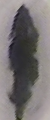
\includegraphics[height=\frameHeight]{dataset/1.png}
%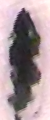
\includegraphics{dataset/2.png}
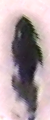
\includegraphics[height=\frameHeight]{dataset/3.png}
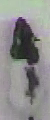
\includegraphics[height=\frameHeight]{dataset/4.png}
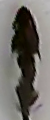
\includegraphics[height=\frameHeight]{dataset/5.png}
%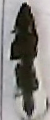
\includegraphics{dataset/6.png}
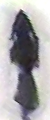
\includegraphics[height=\frameHeight]{dataset/7.png}
\end{center}
\caption{Example of different individuals from the dataset showing the variation in lighting, size, and coloration. These images were taken taken from video sequences in a consistent pose, walking forward, that clearly shows the hood pattern. }
%- show a set of images for different rats (we want to show the variance between rats and changes on the enviroment (eg. variation in illumination)
\end{figure}


\begin{figure}[h]
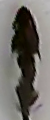
\includegraphics[height=\frameHeight]{dataset/5.png}
\caption{Example of ...}
%- - show a set of images for the same rat and different views
\end{figure}

Description of the data, what criteria we used and how we selected them.

\section{Preliminary Results}
\label{sec:results}

% explain three methods briefly   wang2004image   zhang2011fsim   belongie2002shape

As aforementioned, one approach is to make use of the shape of the hood as a biometric marker. Hence, we used a shape matching technique \cite{belongie2002shape} that, for each shape, finds globally discriminate points, solves the correspondence problem between points in two distinct shapes and estimates an aligning transform between them. The cost for this transformation and the distance between corresponding points are used together as the measure of similarity.

For the appearance based method, we consider the following two quality metrics:

Structure similarity (SSIM)\cite{wang2004image} is used for measuring the similarity between two images. The principle idea is that human visual system is highly sensitive to the structural distortions and automatically compensates for nonstructural distortions (a change of luminance or brightness, a change of contrast and a spatial shift). This method was proposed to capture the image structure distortion. 
It assumes that the original image signals have strong neighbor dependencies which are carrying important information about the structures of the object. This method compares local patterns of pixel intensities that have been normalized for luminance and contrast. Suppose that $x$ and $y$ are local image patches that taken from corresponding location of two compared images. The local SSIM index measures the similarities of three elements of the image patches: the similarity $l(x,y)$ of local patch luminances, the similarity $c(x,y)$ of the localparch contrasts, and the similarity of the local patch structures. These local similarities are combined together to form SSIM. 

Feature similarity (FSIM) \cite{zhang2011fsim} is also proposed to measure image quality according to salient low-level features: phase congruency (PC) and gradient magnitude (GM). PC is a constrast-invariant and dimensionless measure of significance of a local structure, and GM is computed as the secondary feature to encode contrast information. PC and GM are complementary and they reflect different aspects of the HVS in assessing the local quality of the input image. 


Results:

We have 100 testing images. We compare each testing image with all the images in the dataset using shape matching technique \cite{belongie2002shape}, SSIM \cite{wang2004image} and FSIM \cite{zhang2011fsim}. For shape matching technique, the one rat from dataset with minimum cost (or the first 5 rats from dataset with minimum cost) is considered as the correct rat id; for SSIM and FSIM, we consider the first one (or 5) largest value.

\section{Conclusion}
\label{sec:conclusion}
%\blindtext





% use section* for acknowledgement
\section*{Acknowledgment}


The authors would like to thank...


% Can use something like this to put references on a page
% by themselves when using endfloat and the captionsoff option.
\ifCLASSOPTIONcaptionsoff
  \newpage
\fi

\bibliography{bibliography}
\bibliographystyle{ieeetr}


% that's all folks
\end{document}



